\chapter{Cônes de lumière, géodésiques et horizon de Schwarzschild}

Le problème de l’horizon commence par une distinction déjà présente en relativité restreinte. Deux événements voisins peuvent être séparés selon une direction de genre temps, de genre espace ou de genre lumière. La courbure n’abolit pas cette classification. Elle fait du cône de lumière un objet local, différent en chaque événement, et rend la métrique elle-même dynamique. Une fois la métrique connue, le mouvement d’une particule en chute libre découle du même principe du temps propre qui décrit une particule relativiste libre dans un espace-temps plat.

Nous appliquerons ce principe à deux reprises. Il doit d’abord restituer le mouvement newtonien dans un champ faible. Nous l’appliquerons ensuite à la métrique de Schwarzschild, où la signification du temps, de la distance radiale et de la vitesse devient étonnamment subtile.

\section{Intervalles de genre temps, de genre espace et de genre lumière}

Dans un espace-temps plat, avec \(c=1\), l’élément de temps propre est
\begin{equation}
d\tau^2=dt^2-dx^2-dy^2-dz^2.
\label{eq:l5-minkowski-proper-time}
\end{equation}
Rétablir \(c\) est utile dès qu’une approximation non relativiste est proche :
\begin{equation}
d\tau^2
=dt^2-\frac{dx^2+dy^2+dz^2}{c^2}.
\label{eq:l5-minkowski-c}
\end{equation}
La notation \(d\tau^2\) ne garantit pas que le membre de droite soit positif. Son signe classe le déplacement :
\begin{align}
d\tau^2>0
&\quad\Longleftrightarrow\quad \text{time-like},\\
d\tau^2=0
&\quad\Longleftrightarrow\quad \text{light-like},\\
d\tau^2<0
&\quad\Longleftrightarrow\quad \text{space-like}.
\end{align}
Pour un déplacement de genre espace, il est commode de définir la distance propre positive
\begin{equation}
ds^2=-d\tau^2
=dx^2+dy^2+dz^2-dt^2
\qquad(c=1).
\label{eq:l5-proper-distance}
\end{equation}

Le cône de lumière organise ces trois possibilités. Sa surface, et non son intérieur, est constituée des directions de genre lumière. Les directions de genre temps se trouvent à l’intérieur du cône et celles de genre espace à l’extérieur. Les moitiés supérieure et inférieure représentent les cônes de lumière passé et futur.

\begin{figure}[htbp]
\centering
\includegraphics[width=0.82\textwidth]{lecture_05_figure_02.png}
\caption{Temps propre, distance propre et cône causal réunis au tableau. Les rayons lumineux se trouvent sur le cône lui-même ; son intérieur est de genre temps et son extérieur de genre espace.}
\lectureframe{00:05:44}
\end{figure}

\begin{figure}[htbp]
\centering
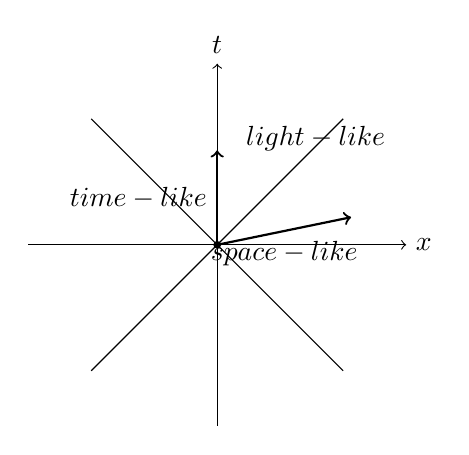
\begin{tikzpicture}[scale=1.0]
\draw[->] (0,-2.3) -- (0,2.3) node[above] {\(t\)};
\draw[->] (-2.4,0) -- (2.4,0) node[right] {\(x\)};
\draw (-1.6,1.6) -- (0,0) -- (1.6,1.6);
\draw (-1.6,-1.6) -- (0,0) -- (1.6,-1.6);
\fill (0,0) circle (1.4pt);
\draw[->,thick] (0,0) -- (0,1.2)
  node[midway,left] {\(\text{time-like}\)};
\draw[->,thick] (0,0) -- (1.7,0.35)
  node[midway,below] {\(\text{space-like}\)};
\node at (1.25,1.35) {\(\text{light-like}\)};
\end{tikzpicture}
\caption{Classification causale dans une section bidimensionnelle de l’espace-temps.}
\end{figure}

Ces intervalles sont opérationnels. Le temps propre est celui qu’indique une horloge transportée le long d’une ligne d’univers de genre temps. La distance propre est celle que mesure un ensemble approprié de règles graduées entre des événements séparés selon une direction de genre espace. Ce ne sont pas de simples noms donnés aux signes d’une forme quadratique.

\section{Signature lorentzienne et un cône en chaque événement}

Avec la convention tensorielle « surtout plus », la métrique plate a pour composantes
\begin{equation}
\eta_{\mu\nu}=\operatorname{diag}(-1,1,1,1),
\label{eq:l5-eta}
\end{equation}
et
\begin{equation}
d\tau^2=-\eta_{\mu\nu}\,dx^\mu dx^\nu.
\label{eq:l5-proper-time-eta}
\end{equation}
La matrice affichée est l’expression d’un tenseur de rang deux dans une base particulièrement simple. Sa caractéristique invariante est sa signature : une direction négative et trois directions positives,
\begin{equation}
\operatorname{signature}(\eta)=(-,+,+,+).
\label{eq:l5-lorentz-signature}
\end{equation}
Une métrique comportant deux signes négatifs aurait deux directions temporelles. De telles signatures peuvent être étudiées mathématiquement, mais elles ne décrivent pas l’espace-temps considéré ici.

Dans un espace-temps courbe, les composantes varient :
\begin{equation}
g_{\mu\nu}=g_{\mu\nu}(x).
\label{eq:l5-position-metric}
\end{equation}
En chaque événement, la métrique doit néanmoins conserver une signature lorentzienne. Chaque événement possède donc ses propres directions de genre temps, sa frontière de genre lumière et ses directions de genre espace. Dans un dessin en coordonnées, les cônes peuvent sembler inclinés ou aplatis différemment d’un point à l’autre, mais la classification causale demeure.

\begin{figure}[htbp]
\centering
\includegraphics[width=0.86\textwidth]{lecture_05_figure_03.png}
\caption{La métrique dépendant de la position \(g_{\mu\nu}(x)\), les étiquettes causales et des esquisses de cônes de lumière locaux.}
\lectureframe{00:09:41}
\end{figure}

\begin{figure}[htbp]
\centering
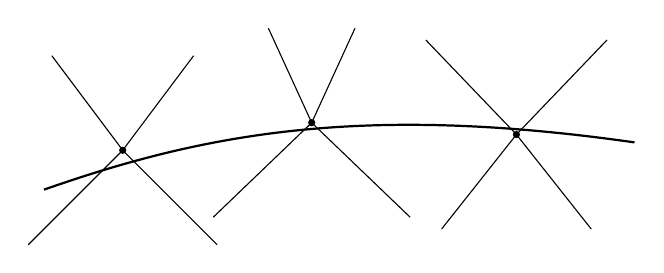
\begin{tikzpicture}[scale=1.0]
\draw[thick] (-4,-0.5) .. controls (-2,0.2) and (0,0.6) .. (3.5,0.1);
\foreach \x/\y/\a/\b in {-3/0/0.9/1.2, -0.6/0.35/0.55/1.25,
                          2.0/0.2/1.15/0.95} {
  \fill (\x,\y) circle (1.3pt);
  \draw (\x,\y) -- ++(-\a,1.2);
  \draw (\x,\y) -- ++(\a,1.2);
  \draw (\x,\y) -- ++(-\b,-1.2);
  \draw (\x,\y) -- ++(\b,-1.2);
}
\end{tikzpicture}
\caption{Cônes locaux voisins. Leur forme en coordonnées peut varier sans changer les vecteurs de genre temps, de genre lumière ou de genre espace.}
\end{figure}

\begin{classroomqa}
\audiencequestion{La valeur propre négative unique sélectionne-t-elle une direction temporelle unique ?}
\lecturerresponse{Une base qui diagonalise la matrice affichée possède une direction de base négative, mais cela ne sélectionne ni observateur privilégié ni flèche physique unique. Les transformations de Lorentz mélangent la coordonnée temporelle aux coordonnées spatiales, et tout vecteur situé à l’intérieur du cône est de genre temps. L’objet invariant est le cône associé à la signature une direction négative et trois positives, et non un vecteur de genre temps distingué.
\lecturetimestamp{00:12:17--00:17:24}}
\end{classroomqa}

\begin{classroomqa}
\audiencequestion{Pourquoi deux dessins du cône local peuvent-ils avoir des formes différentes ?}
\lecturerresponse{Les coordonnées peuvent modifier le dessin. Par exemple, remplacer \(x\) par une coordonnée redimensionnée modifie la pente numérique attribuée à un rayon lumineux et fait donc paraître le cône plus étroit ou plus large. Des coordonnées plus générales peuvent l’incliner. Il s’agit de représenter le même événement et les mêmes relations causales. Dans un espace-temps courbe, les cônes en des événements distincts appartiennent aussi à des espaces tangents distincts ; les comparer exige donc la métrique et une règle de transport.
\lecturetimestamp{00:13:37--00:15:59}}
\end{classroomqa}

\section{Les géodésiques comme problème variationnel}

Une particule libre suit une géodésique de l’espace-temps. Sous forme différentielle, avec un paramètre affine \(\lambda\),
\begin{equation}
\frac{d^2x^\mu}{d\lambda^2}
+\Gamma^\mu{}_{\rho\sigma}
\frac{dx^\rho}{d\lambda}
\frac{dx^\sigma}{d\lambda}=0.
\label{eq:l5-geodesic}
\end{equation}
La connexion indique au vecteur tangent comment rester parallèle à lui-même au cours du mouvement de la particule.

Il existe une deuxième formulation, souvent plus facile à utiliser pour les calculs. Dans un espace riemannien muni de la métrique \(g_{mn}\), la longueur d’une courbe est
\begin{equation}
s=\int ds
=\int\sqrt{g_{mn}\,dx^m dx^n}.
\label{eq:l5-spatial-length}
\end{equation}
La géodésique rend cette longueur stationnaire sous de petites variations du chemin à extrémités fixes. L’intégrale est simplement la somme des longueurs infinitésimales le long de la courbe, et son équation d’Euler--Lagrange est une équation différentielle du second ordre, analogue par sa forme à une loi de force.

Pour une ligne d’univers de genre temps, la longueur spatiale est remplacée par le temps propre :
\begin{equation}
\tau
=\int\sqrt{-g_{\mu\nu}\,dx^\mu dx^\nu}.
\label{eq:l5-proper-time-functional}
\end{equation}
Une géodésique de genre temps rend \(\tau\) stationnaire et, pour des trajectoires de chute libre voisines avant l’apparition de points conjugués, localement maximale. En multipliant par \(-m\), on obtient l’action de la particule
\begin{equation}
A=-m\tau
=-m\int\sqrt{-g_{\mu\nu}\,dx^\mu dx^\nu}.
\label{eq:l5-particle-action}
\end{equation}
Le même trajet minimise donc localement \(A=-m\tau\). La distinction entre un temps propre stationnaire et le signe de l’action choisie lève l’apparente ambiguïté entre minimum et maximum.

\section{Du temps propre au lagrangien usuel}

L’action de \eqref{eq:l5-particle-action} est géométrique, mais on peut la mettre sous la forme familière utilisée en mécanique. Paramétrons la ligne d’univers par la coordonnée \(t\), divisons chaque différentielle par \(dt\) et sortons de la racine le facteur restant \(dt\) :
\begin{align}
A
&=-m\int\sqrt{-g_{\mu\nu}(x)\,dx^\mu dx^\nu}\\
&=-m\int
\sqrt{-g_{\mu\nu}(x)
\frac{dx^\mu}{dt}\frac{dx^\nu}{dt}}\,dt.
\label{eq:l5-action-t}
\end{align}
Pour la composante temporelle, \(dt/dt=1\) ; les composantes spatiales sont les vitesses coordonnées usuelles. Nous pouvons donc écrire
\begin{equation}
\begin{aligned}
A&=\int L\,dt,\\
L&=-m\sqrt{-g_{\mu\nu}(x)\dot x^\mu\dot x^\nu},\\
\dot x^\mu&=\frac{dx^\mu}{dt}.
\end{aligned}
\label{eq:l5-relativistic-lagrangian}
\end{equation}

\begin{figure}[htbp]
\centering
\includegraphics[width=0.88\textwidth]{lecture_05_figure_05.png}
\caption{L’action de la ligne d’univers mise sous la forme usuelle \(A=\int L\,dt\).}
\lectureframe{00:27:00}
\end{figure}

\begin{figure}[htbp]
\centering
\includegraphics[width=0.88\textwidth]{lecture_05_figure_06.png}
\caption{Un état ultérieur du tableau où le lagrangien relativiste est isolé.}
\lectureframe{00:28:59}
\end{figure}

\begin{classroomqa}
\audiencequestion{Les indices d’espace-temps de cette action devraient-ils être grecs ?}
\lecturerresponse{Oui. Les indices grecs parcourent le temps et toutes les coordonnées spatiales. On peut réserver les indices latins aux coordonnées spatiales lorsque cette distinction est utile.
\lecturetimestamp{00:25:53--00:26:03}}
\end{classroomqa}

\begin{classroomqa}
\audiencequestion{Pourquoi appelle-t-on l’expression sous la racine le lagrangien ?}
\lecturerresponse{Une fois l’action écrite sous la forme \(A=\int L\,dt\), l’intégrande est le lagrangien. Ce n’est pas seulement une définition : la variation de cet intégrande donne les équations d’Euler--Lagrange
\[
\frac{d}{dt}
\left(\frac{\partial L}{\partial\dot x^\mu}\right)
=\frac{\partial L}{\partial x^\mu},
\]
qui sont équivalentes à l’équation des géodésiques, à condition de traiter la paramétrisation de façon cohérente.
\lecturetimestamp{00:28:36--00:29:02}}
\end{classroomqa}

Pour une particule massive, la ligne d’univers est de genre temps ; la quantité sous la racine est donc positive. Un trajet de genre espace décrirait un mouvement supraluminique, et non la trajectoire d’une particule massive ordinaire. Une fois la métrique connue, on peut obtenir la trajectoire de la particule soit en calculant les symboles de Christoffel et en utilisant \eqref{eq:l5-geodesic}, soit en appliquant les équations d’Euler--Lagrange à \eqref{eq:l5-relativistic-lagrangian}. Démontrer leur équivalence est un exercice utile ; la méthode de l’action est généralement plus courte.

\section{La limite newtonienne}

Considérons le champ gravitationnel faible et statique à l’extérieur d’une source sphérique. Partons de l’espace-temps plat et autorisons le coefficient de \(dt^2\) à différer légèrement de un :
\begin{equation}
d\tau^2
=\left(1+\frac{2u(\mathbf{x})}{c^2}\right)dt^2
-\frac{d\mathbf{x}^2}{c^2},
\label{eq:l5-weak-metric}
\end{equation}
où \(u\) doit devenir le potentiel newtonien. Cet ansatz doit être vérifié, et pas simplement nommé.

L’action de la particule, avec ses dimensions physiques, est
\begin{equation}
A=-mc^2\int
\sqrt{1+\frac{2u}{c^2}
-\frac{\dot{\mathbf{x}}^{\,2}}{c^2}}\,dt.
\label{eq:l5-weak-action}
\end{equation}
\(u/c^2\) et \(\dot{\mathbf{x}}^{\,2}/c^2\) sont tous deux petits. En conservant leurs contributions au premier ordre,
\begin{equation}
\sqrt{1+\epsilon}
=1+\frac{\epsilon}{2}+O(\epsilon^2),
\qquad
\epsilon=\frac{2u-\dot{\mathbf{x}}^{\,2}}{c^2},
\end{equation}
on obtient
\begin{align}
L
&=-mc^2
\sqrt{1+\frac{2u-\dot{\mathbf{x}}^{\,2}}{c^2}}\\
&=-mc^2-mu+\frac{m}{2}\dot{\mathbf{x}}^{\,2}\\
&\quad+O\!\left(c^{-2}
 [u^2+u\dot{\mathbf{x}}^{\,2}+\dot{\mathbf{x}}^{\,4}]\right).
\label{eq:l5-newton-expansion}
\end{align}
Le terme constant d’énergie de masse au repos n’a aucun effet sur les équations du mouvement. Il reste
\begin{equation}
L_{\mathrm{nr}}
=\frac{m}{2}\dot{\mathbf{x}}^{\,2}-m u(\mathbf{x}),
\label{eq:l5-newton-lagrangian}
\end{equation}
et, par conséquent,
\begin{equation}
m\ddot{\mathbf{x}}=-m\boldsymbol{\nabla}u.
\label{eq:l5-newton-equation}
\end{equation}
La masse d’épreuve se simplifie, comme l’exige la chute libre universelle. L’énergie potentielle est \(m u\), tandis que l’accélération est indépendante de \(m\).

Nous avons ainsi identifié la relation dominante en champ faible
\begin{equation}
g_{00}=1+\frac{2u}{c^2}+O(c^{-4}).
\label{eq:l5-g00-newton}
\end{equation}
À l’extérieur d’une masse sphérique \(M\),
\begin{equation}
u(r)=-\frac{GM}{r},
\qquad
g_{00}=1-\frac{2GM}{rc^2}+O(c^{-4}).
\label{eq:l5-g00-spherical}
\end{equation}
Cela détermine la première correction à la composante temporelle. Cela ne détermine pas encore la métrique complète en champ fort.

\section{Coordonnées sphériques et première conjecture de Schwarzschild}

Les coordonnées sphériques sont naturelles pour une source centrale. Dans le cours, \(\theta\) est mesuré depuis le plan équatorial plutôt que depuis le pôle ; l’élément de ligne angulaire est donc
\begin{equation}
d\Omega^2=d\theta^2+\cos^2\theta\,d\phi^2.
\label{eq:l5-angular-metric}
\end{equation}
Avec cette convention,
\begin{equation}
d\mathbf{x}^2=dr^2+r^2d\Omega^2.
\label{eq:l5-flat-spherical}
\end{equation}
Aucune grandeur physique ne dépend du choix de cette coordonnée \(\theta\), analogue à la latitude ; avec l’angle polaire plus courant, \(\cos^2\theta\) serait remplacé par \(\sin^2\theta\).

Insérer le coefficient temporel newtonien tout en laissant la métrique spatiale plate donne cette première conjecture :
\begin{equation}
\begin{aligned}
d\tau^2
&=\left(1-\frac{r_s}{r}\right)dt^2
-\frac{1}{c^2}\left(dr^2+r^2d\Omega^2\right),\\
r_s&=\frac{2GM}{c^2}.
\end{aligned}
\label{eq:l5-naive-schwarzschild}
\end{equation}
Ce ne peut pas être la réponse exacte. Pour \(r<r_s\), le coefficient de \(dt^2\) change de signe alors que tous les coefficients spatiaux restent négatifs dans la convention du temps propre. La métrique perdrait sa signature une direction temporelle et trois directions spatiales.

Les équations de champ dans le vide fournissent le coefficient radial requis :
\begin{equation}
\boxed{
d\tau^2
=\left(1-\frac{r_s}{r}\right)dt^2
-\frac{dr^2}{c^2\left(1-r_s/r\right)}
-\frac{r^2}{c^2}d\Omega^2.
}
\label{eq:l5-schwarzschild}
\end{equation}
C’est la métrique extérieure de Schwarzschild. Lorsque \(r\) franchit \(r_s\), les coefficients \(t\) et \(r\) changent de signe ensemble, préservant ainsi la signature lorentzienne. En coordonnées de Schwarzschild, la coordonnée radiale devient de genre temps à l’intérieur et la coordonnée \(t\) devient de genre espace. Cet échange signale une défaillance de la carte de coordonnées à l’horizon, et non une défaillance locale de la géométrie de l’espace-temps.

\begin{classroomqa}
\audiencequestion{Combien de temps un objet en chute met-il à franchir l’horizon ?}
\lecturerresponse{Selon la coordonnée de Schwarzschild \(t\) utilisée par un observateur lointain, le franchissement est repoussé à un temps infini. Selon le temps propre indiqué par l’horloge de l’objet en chute, il se produit en un temps fini. La distinction entre ces horloges est le problème central de l’horizon.
\lecturetimestamp{00:54:45--00:55:35}}
\end{classroomqa}

\begin{classroomqa}
\audiencequestion{Pourquoi modifier le coefficient radial plutôt qu’une autre partie de la métrique ?}
\lecturerresponse{La métrique doit conserver sa signature lorentzienne, la symétrie sphérique distingue la direction radiale de la sphère angulaire et les équations de champ dans le vide déterminent précisément le facteur réciproque. La signature indique où chercher ; les équations d’Einstein donnent le résultat exact.
\lecturetimestamp{00:55:35--00:56:01}}
\end{classroomqa}

Pour la Terre, \(r_s\) n’est que de l’ordre du centimètre, profondément enfoui dans le corps matériel. La métrique extérieure du vide n’y est pas valable ; la Terre n’a donc pas d’horizon de Schwarzschild. À l’intérieur de la matière, il faut la remplacer par une solution intérieure et raccorder celle-ci à la surface.

\begin{classroomqa}
\audiencequestion{Si \(t\) et \(r\) échangent leurs rôles de coordonnées, qu’advient-il d’une horloge ordinaire ?}
\lecturerresponse{L’horloge continue de mesurer le temps propre le long d’une ligne d’univers de genre temps. Elle ne sait pas qu’une coordonnée choisie est devenue malcommode. Un système de coordonnées régulier associé à la chute libre montre une géométrie locale régulière et une propagation locale ordinaire de la lumière à travers l’horizon.
\lecturetimestamp{00:56:35--00:57:50}}
\end{classroomqa}

\subsection{Pourquoi la correction radiale n’apparaissait pas dans l’équation de Newton}

La métrique exacte modifie le coefficient radial dès le premier ordre en le potentiel :
\begin{equation}
\frac{1}{1-r_s/r}
=1+\frac{r_s}{r}
+O\!\left(\frac{r_s^2}{r^2}\right)
=1-\frac{2u}{c^2}+O(c^{-4}).
\label{eq:l5-radial-expansion}
\end{equation}
Pourquoi était-il légitime d’ignorer cette modification dans la dérivation newtonienne ? Dans l’action de la particule, elle multiplie \(\dot r^2/c^2\). Sa première correction est donc proportionnelle à
\begin{equation}
\frac{u\,\dot r^2}{c^4},
\end{equation}
ce qui dépasse l’ordre conservé dans \eqref{eq:l5-newton-expansion}. La correction radiale est négligeable pour le test newtonien à faible vitesse, mais elle devient déterminante pour le mouvement relativiste et près de l’horizon. Cela rappelle utilement qu’un terme trop petit pour une approximation donnée peut gouverner le phénomène qui nous intéresse dans une autre.

\section{Chute radiale en temps de Schwarzschild}

Posons \(c=1\) et étudions d’abord le mouvement radial. Les orbites circulaires sont également importantes, mais elles nécessitent les termes angulaires et seront abordées plus tard. Le mouvement radial ressemble moins à une orbite qu’à une chute directe vers la source ; il met en évidence le comportement de l’horizon avec le moins de calculs.

\begin{classroomqa}
\audiencequestion{De quel temps dépend la vitesse radiale ?}
\lecturerresponse{Le point au-dessus de la variable indique une dérivée par rapport au temps coordonné de Schwarzschild \(t\), normalisé par l’observateur statique lointain. La montre de l’observateur en chute mesure le temps propre \(\tau\). Confondre les deux transformerait un énoncé sur les coordonnées en un faux énoncé local.
\lecturetimestamp{01:04:03--01:04:47}}
\end{classroomqa}

Pour \(d\Omega=0\), définissons
\begin{equation}
a(r)=1-\frac{r_s}{r}.
\label{eq:l5-a-def}
\end{equation}
La métrique et le lagrangien radiaux sont
\begin{align}
d\tau^2&=a\,dt^2-\frac{dr^2}{a},\\
L&=-m\sqrt{a-\frac{\dot r^2}{a}},
\qquad
\dot r=\frac{dr}{dt}.
\label{eq:l5-radial-lagrangian}
\end{align}
Comme \(L\) ne dépend pas explicitement de \(t\), son hamiltonien est conservé. La quantité de mouvement radiale est
\begin{equation}
p_r=\frac{\partial L}{\partial\dot r}
=\frac{m\dot r}{a\sqrt{a-\dot r^2/a}},
\label{eq:l5-radial-momentum}
\end{equation}
et
\begin{align}
H
&=p_r\dot r-L\\
&=\frac{ma}{\sqrt{a-\dot r^2/a}}
=E.
\label{eq:l5-radial-energy}
\end{align}
En isolant la vitesse coordonnée, on obtient
\begin{equation}
\boxed{
\dot r^2
=a^2\left(1-\frac{m^2}{E^2}a\right).
}
\label{eq:l5-radial-velocity}
\end{equation}
Le calcul au tableau examine plusieurs formes algébriques intermédiaires ; l’expression encadrée est le résultat cohérent.

Lorsque \(r\) tend vers \(r_s\), \(a(r)\) tend vers zéro tandis que le facteur entre parenthèses tend vers un. Par conséquent,
\begin{equation}
\frac{dr}{dt}
\sim -\left(1-\frac{r_s}{r}\right)
\longrightarrow 0
\qquad(r\longrightarrow r_s^+)
\label{eq:l5-infall-freeze}
\end{equation}
pour une particule entrante. En temps de Schwarzschild, la particule semble ralentir et se figer juste à l’extérieur de l’horizon.

\begin{classroomqa}
\audiencequestion{La diminution de \(dr/dt\) signifie-t-elle que la gravité est devenue répulsive ?}
\lecturerresponse{Non. La particule n’est pas poussée localement vers l’extérieur. La coordonnée \(t\) devient de moins en moins adaptée à la description du franchissement, si bien que le déplacement radial par unité de \(t\) tend vers zéro. L’accélération propre le long de la ligne d’univers en chute libre reste nulle et l’horizon est atteint en un temps propre fini.
\lecturetimestamp{01:14:18--01:16:38}}
\end{classroomqa}

En effet, près de l’horizon,
\begin{equation}
\frac{dt}{dr}
\sim-\frac{1}{1-r_s/r}
=-\frac{r}{r-r_s}.
\end{equation}
Son intégrale diverge logarithmiquement. Cela démontre que le temps de Schwarzschild est infini sans impliquer que l’horloge de l’objet en chute indique un temps infini.

\section{Rayons lumineux radiaux}

Le cas de la lumière donne la version la plus courte du même calcul. Pour un rayon lumineux radial nul,
\begin{equation}
d\tau^2
=a\,dt^2-\frac{dr^2}{a}=0.
\end{equation}
On obtient donc
\begin{equation}
\boxed{
\frac{dr}{dt}
=\pm a(r)
=\pm\left(1-\frac{r_s}{r}\right).
}
\label{eq:l5-radial-light}
\end{equation}
Le signe plus décrit un rayon sortant et le signe moins un rayon entrant. Les deux vitesses coordonnées tendent vers zéro à l’horizon.

\begin{classroomqa}
\audiencequestion{Quelle vitesse la formule donne-t-elle loin de la source ?}
\lecturerresponse{Lorsque \(r\) tend vers l’infini, \(a(r)\) tend vers un, donc \(dr/dt\) tend vers \(\pm1\), ou \(\pm c\) lorsque les unités sont rétablies.
\lecturetimestamp{01:21:01--01:21:29}}
\end{classroomqa}

La relativité générale fonctionne souvent ainsi : les principes tiennent en quelques lignes, tandis que les coordonnées et les calculs deviennent compliqués. L’équation \eqref{eq:l5-radial-light} est simple, mais il faut interpréter avec soin sa valeur qui s’annule près de \(r_s\). C’est une vitesse coordonnée, et non la vitesse mesurée par un observateur inertiel local.

\section{Ce qu’observe un observateur lointain}

\begin{classroomqa}
\audiencequestion{La lumière émise près de l’horizon peut-elle s’en échapper, et s’agit-il du rayonnement de Hawking ?}
\lecturerresponse{Un rayon classique sortant, émis juste à l’extérieur de l’horizon, peut se déplacer vers l’extérieur, mais sa vitesse coordonnée de Schwarzschild est initialement extrêmement faible et le signal n’atteint l’infini qu’après un retard et un décalage vers le rouge considérables. Dans ces coordonnées, un rayon situé sur l’horizon y reste ; un rayon situé à l’intérieur ne peut pas s’échapper. Le rayonnement de Hawking est un effet de théorie quantique des champs associé à la géométrie extérieure, et non un rayon lumineux classique remontant depuis l’intérieur ; le calcul présenté ici ne le dérive pas.
\lecturetimestamp{01:22:08--01:24:28}}
\end{classroomqa}

\begin{classroomqa}
\audiencequestion{Si un photon semble presque immobile, commence-t-il à paraître massif ?}
\lecturerresponse{Non. Un observateur local en chute libre mesure toujours le photon à la vitesse \(c\). Seul le rapport coordonné \(dr/dt\) tend vers zéro. La masse, le caractère nul et la vitesse locale de la lumière ne sont pas modifiés par une carte de coordonnées mal adaptée.
\lecturetimestamp{01:24:31--01:25:26}}
\end{classroomqa}

L’expression de Schwarzschild utilisée ici est une solution extérieure dans le vide. Une étoile, une planète ou un nuage en effondrement possède une métrique intérieure différente, qu’il faut raccorder à celle-ci. Si la surface matérielle reste à l’extérieur de \(r_s\), comme c’est le cas pour la Terre, qui en est très éloignée, l’horizon coordonné extérieur se trouve hors du domaine où la formule du vide peut être prolongée à travers la matière. Si le corps s’effondre à l’intérieur de son rayon de Schwarzschild, l’horizon fait partie de l’espace-temps physique.

\begin{classroomqa}
\audiencequestion{Si un observateur extérieur ne voit jamais la matière franchir l’horizon, comment un trou noir peut-il se former ou croître ?}
\lecturerresponse{Le raisonnement traite le temps de Schwarzschild comme s’il s’agissait d’une horloge physique globale à l’horizon. La conclusion selon laquelle un trou noir ne pourrait donc jamais croître semble plausible, mais elle est fausse. Une réponse complète exige des coordonnées régulières qui traversent l’horizon et la géométrie causale globale de l’effondrement ; cette résolution sera abordée à la prochaine étape du cours.
\lecturetimestamp{01:27:57--01:29:36}}
\end{classroomqa}

\begin{classroomqa}
\audiencequestion{Que mesurerait un radar routier pour une voiture qui tombe vers l’horizon ?}
\lecturerresponse{La vitesse coordonnée augmente d’abord lorsque la voiture tombe, puis atteint un maximum et décroît vers zéro. Des impulsions radar envoyées plus tard peuvent encore atteindre la voiture à l’extérieur de l’horizon, mais leur aller-retour prend progressivement plus de temps. Le signal renvoyé subit un décalage vers le rouge de plus en plus important, et l’image semble ralentie et comprimée près de \(r_s\). Ce n’est pas une représentation locale fiable de l’expérience du conducteur ; celui-ci franchit l’horizon en un temps propre fini.
\lecturetimestamp{01:29:39--01:32:14}}
\end{classroomqa}

\begin{classroomqa}
\audiencequestion{La vitesse de la lumière est-elle constante uniquement en relativité restreinte ?}
\lecturerresponse{Elle est également constante dans chaque référentiel inertiel local de la relativité générale. Un observateur en chute, muni d’horloges et de règles graduées locales, mesure la vitesse d’un photon proche à \(c\). Les vitesses coordonnées comme \(dr/dt\) peuvent varier parce que \(r\) et \(t\) ne correspondent pas aux mesures d’un même laboratoire inertiel local dans tout l’espace-temps.
\lecturetimestamp{01:32:20--01:34:20}}
\end{classroomqa}

\section{Questions au-delà du calcul de Schwarzschild}

\begin{classroomqa}
\audiencequestion{Que pourrait signifier l’unification de la gravité avec les autres interactions ?}
\lecturerresponse{Une possibilité géométrique consiste à étendre l’espace-temps par des dimensions compactes supplémentaires. Des composantes d’une métrique de dimension supérieure peuvent alors apparaître en quatre dimensions sous forme de champs de jauge et de champs scalaires, tandis que la quantité de mouvement dans une dimension supplémentaire peut se manifester comme une charge. C’est une piste structurelle associée aux idées de Kaluza--Klein, et non une unification achevée dans le présent cours.
\lecturetimestamp{01:34:22--01:36:08}}
\end{classroomqa}

\begin{classroomqa}
\audiencequestion{Des régions ou des univers différents pourraient-ils avoir des signatures métriques différentes ?}
\lecturerresponse{La relativité générale classique fixe ordinairement une signature lorentzienne non dégénérée. La modifier exigerait que la métrique passe par une configuration dégénérée, où la description classique standard échoue. La gravité quantique pourrait imposer un cadre plus général, mais aucune théorie établie présentée ici ne prédit des régions physiques où la signature change.
\lecturetimestamp{01:36:08--01:38:08}}
\end{classroomqa}

\begin{classroomqa}
\audiencequestion{Comment Schwarzschild a-t-il trouvé cette solution alors qu’il servait pendant la Première Guerre mondiale ?}
\lecturerresponse{La remarque faite en cours est autant humaine qu’historique : Schwarzschild était astronome et mathématicien de grand talent, et travailler sur les nouvelles équations d’Einstein lui offrait un refuge intellectuel au milieu de son service en temps de guerre.
\lecturetimestamp{01:38:11--01:39:02}}
\end{classroomqa}

La leçon centrale est désormais assez claire pour nous guider dans la suite. La métrique détermine à la fois les cônes causaux et le mouvement libre. Sa composante temporelle en champ faible contient le potentiel de Newton, tandis que sa forme exacte de Schwarzschild donne un horizon de coordonnées à \(r=r_s\). Le temps de Schwarzschild étire le franchissement jusqu’à l’infini ; le temps propre de l’observateur en chute, lui, reste fini. Résoudre globalement ce contraste et expliquer comment un trou noir se forme malgré l’image figée pour l’observateur lointain constitue le prochain problème.